% FACT, manuscript for Robotics and Autonomous Systems (Elsevier, elsarticle).
% Build: pdflatex main && bibtex main && pdflatex main && pdflatex main. check_numbers.py checks the numbers;
% highlights.txt holds the highlights, uploaded as a separate file.
\documentclass[preprint,12pt]{elsarticle}
\usepackage[T1]{fontenc}
\usepackage{mathptmx}
\usepackage[scaled=0.92]{helvet}
\usepackage{courier}
\usepackage{amsmath,amssymb,amsthm}
\usepackage{booktabs}
\usepackage{array}
\usepackage{graphicx}
\usepackage{xcolor}
\usepackage{algorithm}
\usepackage{algpseudocode}
\usepackage{tikz}
\usetikzlibrary{arrows.meta,positioning}
\usepackage{lineno}
\usepackage[hidelinks]{hyperref}
\usepackage{xurl}

\setlength{\belowcaptionskip}{4pt}
\newcommand{\todo}[1]{\textcolor{red}{[#1]}}
\newcommand{\method}{FACT}
\newcommand{\E}{\mathbb{E}}
\newcommand{\pmse}[2]{#1{\scriptsize$\pm$#2}}
\newtheorem{proposition}{Proposition}
\newcolumntype{L}[1]{>{\raggedright\arraybackslash}p{#1}}

\journal{Robotics and Autonomous Systems}

\begin{document}

\begin{frontmatter}

\title{\method: Curating Learned Dynamics for MPPI When Most Logs Are Wrong}

\author[ind]{Apurba Bose\fnref{eq}}
\author[ut]{Soovadeep Bakshi\corref{cor}\fnref{eq}}
\ead{soovadeep.bakshi@utexas.edu}
\author[ut]{Jiachen Li}
\author[ut]{Dongmei Chen}
\cortext[cor]{Corresponding author.}
\fntext[eq]{These authors contributed equally to this work.}
\affiliation[ind]{organization={Independent researcher}, city={San Jose}, state={CA}, postcode={95118}, country={USA}}
\affiliation[ut]{organization={Walker Department of Mechanical Engineering, The University of Texas at Austin},
  city={Austin}, state={TX}, postcode={78712}, country={USA}}

\begin{abstract}
MPPI is only as safe as its learned dynamics model, and the model only as good as its logs. Logs can be consistently wrong, for instance recorded before a propeller change. When such a fault covers most logs in a regime, no rule that sees only the logs can reliably identify the wrong group, and a few failures added to training at a fixed weight are outvoted. A short trusted trajectory covering that regime can instead identify the misleading logs, and failures provide one naturally: they record the deployed dynamics where the model is wrong. \method{} (Failure-Anchored Curation of Training logs) scores each training sample by whether fitting it moves the model away from the failure, removes every log with a positive mean score, with no count to tune, and retrains. On a quadrotor simulated from real NeuroBEM logs, with 67\% of the descent data faulty, one crash dive, or a supervisor's takeover, lowers the crash rate from 99\% to 3.1\%; robust fitting leaves 97--98\%, and adding the crash 71--95\%. Learning to reweight with the crash as its clean set completes more dives safely, but crashes more on a thrust-gain fault (9.7\% against 1.9\%) and costs more. Several assumptions fail in other settings: on a battery fault in real Crazyflie logs, curation alone fails and three crashes help mainly as data; on a car whose model cannot represent ice, \method{} is only a regime filter; and a fault that starts mid-flight needs a second failure. All closed-loop tests are simulated.
\end{abstract}

\begin{keyword}
learned dynamics \sep model predictive path integral control \sep data curation \sep training-data attribution \sep failure data \sep quadrotor
\end{keyword}

\end{frontmatter}

\linenumbers

\section{Introduction}\label{sec:intro}

Learned dynamics models let sampling-based model predictive control such as MPPI~\citep{williams2017mppi,williams2017itmpc} fly and drive aggressively, because the planner can exploit effects that a first-principles model misses~\citep{nagabandi2018neural,chua2018pets,shi2019neurallander,torrente2021datadriven,bauersfeld2021neurobem,oconnell2022neuralfly,salzmann2023neuralmpc}. The same exploitation makes the planner fragile: where the model is optimistic, MPPI plans to the edge of what the model allows, and the robot crashes.

A model is optimistic where its logs are wrong, and system-identification logs are often wrong in a consistent way. A fleet's logs pile up across propeller sets, firmware versions and batteries, and a log recorded before a propeller change is a clean recording of a slightly different robot. If such logs make up most of the data in some regime, the learned model is confidently wrong there.

Standard data cleaning trusts the majority: robust losses and small-loss filtering discard what disagrees with the consensus, and models trained on a consistent majority agree, so ensembles see no problem. When faulty and correct logs cover the same states, no rule that sees only the logs can reliably identify which group matches the deployed dynamics (Proposition~\ref{prop:ident}). Data from the deployed robot breaks the tie, and a failure that has happened is such data, from where the model is wrong. But a few failure runs are a few hundred samples against tens of thousands of faulty ones: added at a fixed weight they are outvoted (Proposition~\ref{prop:add}), and they cover only the states the failure visited.

Our observation is that, for such faults, a failure is more useful as an answer key than as training data: it is a trusted record of the regime where the model is wrong, and any such record serves (Section~\ref{sec:ref}). \method{} scores every training sample by whether a gradient step on it would increase the model's error along the failure~\citep{pruthi2020tracin}, removes every log with a positive mean score, and retrains (Fig.~\ref{fig:pipeline}). On a quadrotor whose plant is fit to real NeuroBEM flight logs~\citep{bauersfeld2021neurobem}, with two thirds of the descent data recorded under a propeller fault, the planner crashes in 98.9\% of dives. One crash dive, used by \method{}, brings this to 3.1\%, close to the 1.9\% of a model trained without the faulty logs, while adding the same dive to training leaves 94.7\% (Table~\ref{tab:major}). A run that a safety supervisor takes over before impact serves as well as a crash.

In an idealised setting the sign of \method{}'s score separates the two groups whichever is the majority (Propositions~\ref{prop:sign}--\ref{prop:agg}), and removing the wrong logs fixes the model wherever they covered, not only along the failure. The claim is deliberately narrow: \method{} addresses consistent majority faults in learned dynamics, where faulty and correct logs overlap in state space, using a few closed-loop failures as trusted references for the deployed dynamics; it is not general-purpose data cleaning. A large part of this paper is about where the claim stops. Several assumptions of the analysis fail in our experiments, and Section~\ref{sec:discussion} maps each assumption to where it holds, where it fails and what \method{} does there.

\noindent Our contributions are:
\begin{itemize}
\item An idealised account of why failure-free cleaning cannot remove a consistent wrong majority, why failures added at a fixed weight leave the fault where they do not reach, why a failure used as an attribution target separates the groups, with or without normalisation, and why a log's mean score is reliable where its samples are not; and a measurement of how far a trained network's attribution score is from that account (Section~\ref{sec:analysis}).
\item \method{}, failure-anchored curation of training logs: the failure's transitions are trusted labels of the deployed dynamics, each sample is scored once by gradient alignment with them, logs with a positive mean score are removed, with no count to choose, and the unchanged pipeline retrains, returning an explicit list of logs to inspect; on the quadrotor a gradient-free score that compares errors does nearly as well, so what matters most there is the reference (Sections~\ref{sec:method} and~\ref{sec:scores}).
\item Closed-loop experiments on a quadrotor whose plant is learned from real NeuroBEM logs, a MuJoCo car and a fault in real Crazyflie logs, against failure-free cleaning, location rules, CUPID~\citep{agia2025cupid}, weighted addition, replay fine-tuning and learning to reweight~\citep{ren2018l2rw}, with budget and random-removal controls, other plants, degraded failure records and sweeps over the fault (Section~\ref{sec:results}).
\item An assumption-by-assumption account of where \method{} stops, and practical checks for deciding when to use it (Section~\ref{sec:discussion}).
\end{itemize}

Section~\ref{sec:related} reviews related work, Section~\ref{sec:problem} states the problem, Section~\ref{sec:analysis} analyses it, Section~\ref{sec:method} gives the method, Section~\ref{sec:setup} the experimental setup, Section~\ref{sec:results} the results and Section~\ref{sec:discussion} the discussion; Section~\ref{sec:conclusion} concludes.

\section{Related work}\label{sec:related}

\textbf{Learned dynamics for planning and control.} Neural dynamics models drive model-based control from MPPI with learned models~\citep{williams2017itmpc} and model-based reinforcement learning~\citep{nagabandi2018neural,chua2018pets} to agile quadrotor flight, where they capture ground effect~\citep{shi2019neurallander}, aerodynamic residuals~\citep{torrente2021datadriven,bauersfeld2021neurobem,salzmann2023neuralmpc} and wind~\citep{oconnell2022neuralfly}. \citet{brunke2022safelearning} survey how such models are made safe. These works assume that the logs record the deployed robot, and treat model error as a matter of capacity or coverage. We study what happens when most logs in a regime record a different robot.

\textbf{Adapting to changed dynamics.} Online adaptation and meta-learning adjust a model to current conditions from recent data~\citep{nagabandi2019adapt,oconnell2022neuralfly}. That corrects the model near the states the robot is visiting, which is what fine-tuning on a failure does; we find that this leaves the fault where the failure did not go (Section~\ref{sec:reweight}). Curation removes the wrong logs everywhere they covered, and the two are complementary.

\textbf{Failure-free robustness.} Probabilistic ensembles and uncertainty penalties keep a planner where several learned models agree~\citep{chua2018pets,yu2020mopo}, but disagreement signals too little data, not wrong data: models trained on a consistent fault agree. Robust losses~\citep{huber1964robust}, small-loss sample selection~\citep{han2018coteaching} and confident learning~\citep{northcutt2021confident}, surveyed by \citet{song2023noisylabels}, identify bad labels by their disagreement with the rest of the data. They work when bad labels are a minority or inconsistent, as we confirm, and fail when they are a consistent majority.

\textbf{Reweighting towards trusted data.} Learning to reweight~\citep{ren2018l2rw} weights each minibatch sample, at every step, by the alignment of its gradient with that of a small clean set; Meta-Weight-Net~\citep{shu2019mwn} learns the weighting instead. It is the closest approach to ours, and with a failure run as its clean set it matches \method{} on two of three benchmarks (Section~\ref{sec:reweight}). \method{} differs in its trusted data (the deployed robot's own failure), its unit (whole logs, whose mean score is reliable where single samples are not, Proposition~\ref{prop:agg}), its cost (one scoring pass) and its output (a list of logs to inspect, then ordinary retraining). Fine-tuning with replay of old data~\citep{rolnick2019replay} is the standard way to adapt a model without forgetting; we compare against both.

\textbf{Data attribution and curation in robot learning.} Influence functions~\citep{koh2017influence}, TracIn~\citep{pruthi2020tracin}, datamodels~\citep{ilyas2022datamodels}, TRAK~\citep{park2023trak} and data valuation~\citep{ghorbani2019shapley} estimate how training samples affect a model's predictions. In control they have curated the demonstrations that train controllers for cyber-physical systems~\citep{ifcps2026}, attributed an identified linear model's LQR performance to its identification trajectories~\citep{lqrinfluence2026}, curated the training data of a learned safety predictor for control barrier functions~\citep{dacbf2026}, selected the data columns of data-enabled predictive control~\citep{dmdeepc2025}, and scored MPPI's own sampled rollouts rather than any training data~\citep{dmmppi2025}. None scores the logs that train a dynamics model against the robot's own failure, used as correctly labelled data, and none targets a consistent wrong majority. In robot learning, data quality matters for imitation~\citep{belkhale2023dataquality}, and demonstrations are curated by mutual-information estimates of their quality~\citep{hejna2025demInf}, by datamodels of a target task's loss~\citep{dass2025datamil}, or, in CUPID~\citep{agia2025cupid}, by their influence on closed-loop success. CUPID can curate from failed rollouts alone (its TuckBox task starts at 0\% success), but its practical score is label-free: it measures how much a demonstration resembles the rollouts in gradient space, so it sees where a failure happened, not whether a log's labels are wrong. \method{} uses the failure as correctly labelled data: one run sufficed on our quadrotor benchmarks, with no removal count, and it tells faulty logs from correct ones in the same states, where CUPID from 100 rollouts, told to remove 40, crashes in 39--93\% of dives against 1.4--3.1\% (Section~\ref{sec:main}; our adaptation of CUPID to dynamics models is in \ref{app:protocol}). Crashes have also been collected deliberately as negative examples for learning a policy~\citep{gandhi2017crashing}; we use a failure instead as a reference for the dynamics.

\section{Problem formulation}\label{sec:problem}

A learned model $f_\theta$ maps an input $x$ (state features and command) to a target $y$ (here, the part of the body acceleration that a nominal model does not explain). It is trained by least squares on a set of logs $\mathcal{L}=\{\ell_1,\dots,\ell_M\}$, each a sequence of transitions $(x,y)$. MPPI plans with $f_\theta$ and controls the deployed plant, whose map is $f^\star$. A \emph{failure run} $\tau$ is a closed-loop run that violates a safety constraint, or that a safety supervisor takes over before it does. Its transitions $(x_t,y^\star_t)$ are observations of the deployed dynamics, $y^\star_t=f^\star(x_t)+\text{noise}$. In our experiments the deployed plant is simulated; for the quadrotors it is a model fit to real flight logs.

\textbf{Consistent fault.} In some regime $\mathcal{R}$ (for a drone, fast axial descent), a set of logs $\mathcal{B}$ follows a map $g\neq f^\star$: $y=g(x)+\text{noise}$. The fault is \emph{consistent}: the bad logs agree with each other, so a model can fit them. It is a \emph{majority} fault if the bad logs hold more than half of the data in $\mathcal{R}$. The goal is to find and remove $\mathcal{B}$ from a few failure runs, retrain, and run without crashing on new tasks.

\begin{figure}[t]
\centering
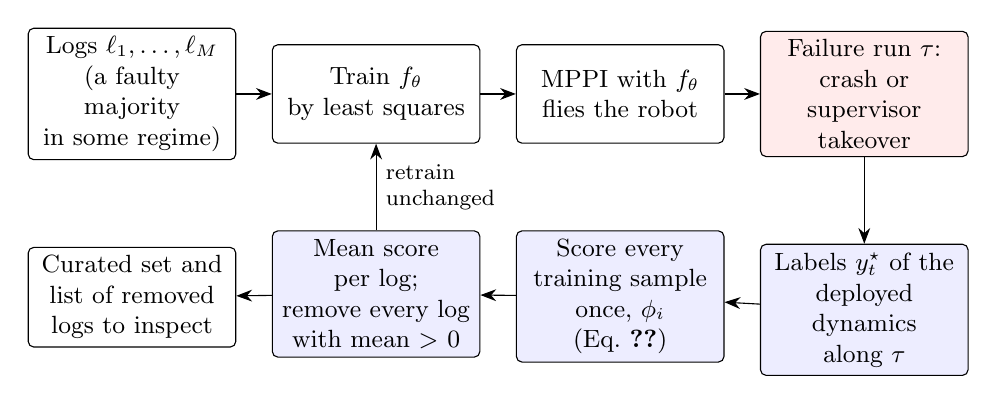
\begin{tikzpicture}[font=\small, >={Stealth[length=2mm]},
  box/.style={draw, rounded corners=2pt, align=center, text width=0.2\textwidth, minimum height=1.25cm, inner sep=3pt},
  hot/.style={box, fill=red!8}, ours/.style={box, fill=blue!7}]
\node[box] (logs) {Logs $\ell_1,\dots,\ell_M$\\ (a faulty majority\\ in some regime)};
\node[box, right=0.45cm of logs] (train) {Train $f_\theta$\\ by least squares};
\node[box, right=0.45cm of train] (mppi) {MPPI with $f_\theta$\\ flies the robot};
\node[hot, right=0.45cm of mppi] (fail) {Failure run $\tau$:\\ crash or supervisor\\ takeover};
\node[ours, below=1.1cm of fail] (lab) {Labels $y^\star_t$ of the\\ deployed dynamics\\ along $\tau$};
\node[ours, below=1.1cm of mppi] (score) {Score every\\ training sample\\ once, $\phi_i$ (Eq.~\ref{eq:score})};
\node[ours, below=1.1cm of train] (rate) {Mean score per log;\\ remove every log\\ with mean $>0$};
\node[box, below=1.1cm of logs] (out) {Curated set and\\ list of removed\\ logs to inspect};
\draw[->] (logs) -- (train);
\draw[->] (train) -- (mppi);
\draw[->] (mppi) -- (fail);
\draw[->] (fail) -- (lab);
\draw[->] (lab) -- (score);
\draw[->] (score) -- (rate);
\draw[->] (rate) -- (out);
\draw[->] (rate.north) -- node[right, align=left, font=\footnotesize] {retrain\\ unchanged} (train.south);
\end{tikzpicture}
\caption{Failure-anchored curation. A failure of the planner (red) records the deployed dynamics where the learned model is wrong. \method{} (blue) uses it as a reference: it scores each training sample by whether training on it moves the model away from the failure, removes the logs whose mean score is positive, and retrains with the unchanged pipeline.}
\label{fig:pipeline}
\end{figure}

\section{Why a deployment reference is needed}\label{sec:analysis}

\subsection{Logs alone, and failures as data}

\begin{proposition}[Logs alone cannot reliably identify the wrong group]\label{prop:ident}
Let the logs in $\mathcal{R}$ come from two groups with label maps $g_1$ and $g_2$, sharing the same input distribution and noise, where group 1 holds a fraction $\rho$ of the data. Consider world~1, where $f^\star=g_2$, and world~2, where $f^\star=g_1$. Any cleaning rule $C$ that sees only the logs and outputs a model $\hat f=C(\mathcal{L})$ satisfies, at every $x\in\mathcal{R}$,
\begin{equation}
\E_1\|\hat f(x)-g_2(x)\|+\E_2\|\hat f(x)-g_1(x)\|\ \ge\ \|g_1(x)-g_2(x)\|.
\end{equation}
So in at least one world its expected error is at least half the gap between the groups. A rule that follows the majority has the full gap as its error in the world where the majority is wrong.
\end{proposition}
\begin{proof}
The logs are generated the same way in both worlds; only which map is the deployed robot differs. So $\hat f(x)$ has the same distribution in both worlds, and the bound is the triangle inequality applied inside one expectation.
\end{proof}
Robust losses, worst-fit filtering and ensembles are all such rules. Any correctly labelled data from the deployed robot in $\mathcal{R}$ breaks the symmetry; a failure is the record a planner produces on its own where its model is wrong (Section~\ref{sec:ref} compares it with other such records). Rules that see \emph{where} a failure happened but not its labels, such as dropping the most crash-like logs or CUPID's label-free surrogate, find bad logs only if no correct look-alike logs cover the same states (Section~\ref{sec:main}).

\begin{proposition}[A fixed weight leaves the fault where failures do not reach]\label{prop:add}
Suppose the model can fit each input separately (a pointwise least-squares fit). At an input with $N_b$ faulty and $N_g$ correct samples, adding $n$ failure transitions with weight $W$ leaves a fraction $N_b/(N_b+N_g+Wn)$ of the fault $g-f^\star$ in the model. At an input the failure runs do not visit ($n=0$) the fraction is $N_b/(N_b+N_g)$ for every $W$. Removing the faulty logs leaves none at any input.
\end{proposition}
Where a failure has data, a large enough weight does fix a pointwise fit; on our drone benchmark (27k faulty against 13k correct descent samples) one crash dive of 94 transitions at $W=20$ still leaves about 64\% of the fault there. Larger weights are limited by coverage: how far a network spreads a heavily weighted fix is empirical (Section~\ref{sec:reweight}).

\subsection{A failure as a reference}

\begin{proposition}[The score's sign separates the groups]\label{prop:sign}
In the setting of Proposition~\ref{prop:ident}, with $\Delta=g_1-g_2$, assume (i) the fit is pointwise least squares, $\hat f=\rho g_1+(1-\rho)g_2$; (ii) the failure run's residual comes from the fault alone, $e_t=\hat f(x_t)-f^\star(x_t)$; (iii) the fault keeps its direction over $\mathcal{R}$, $\langle\Delta(x),\Delta(x')\rangle>0$; and (iv) the score uses a nonnegative scalar kernel, $\phi_i=-\sum_t k(x_t,x_i)\langle e_t,e_i\rangle$ with $e_i=\hat f(x_i)-y_i$, $k\ge0$, and $k(x_t,x_i)>0$ for some $t$. Then, in expectation over label noise, faulty samples have $\phi_i>0$ and correct samples $\phi_i<0$, for every $\rho\in(0,1)$.
\end{proposition}

The sign does not depend on which group is larger: the failure fixes the reference, not the vote (proofs in \ref{app:proofs}). \method{} divides each score by the gradient norm, which can flip the sign of an expectation (\ref{app:proofs}), but not with spherically symmetric noise, two or more outputs and an isotropic Jacobian.

\begin{proposition}[Normalisation keeps the sign]\label{prop:norm}
In the setting of Proposition~\ref{prop:sign}, let $\tilde\phi_i=\phi_i/\|\nabla_\theta l_i\|$ with $\nabla_\theta l_i=J_i^\top e_i$, and assume further (v) the outputs have dimension $d\ge2$, the label noise has a spherically symmetric density, and $J_iJ_i^\top=c_iI$ with $c_i>0$. Then $\E\tilde\phi_i$ has the sign of $\E\phi_i$.
\end{proposition}

\begin{proposition}[A log's mean is reliable where its samples are not]\label{prop:agg}
Let a log's $n$ samples have cosine scores $c_j=\phi_j/\|\nabla L_\tau\|\in[-1,1]$ with mean $\mu=\frac1n\sum_j\E c_j\neq0$, each $\sigma$-sub-Gaussian about its mean ($\sigma\le1$), and $\tau$-dependent: $\{c_j\}_{j\le k}$ is independent of $\{c_j\}_{j\ge k+\tau}$ for every $k$. Then the log's mean score has the sign of $\mu$ except with probability at most $\exp(-n\mu^2/(2\tau\sigma^2))$, while a single sample's chance of the wrong sign does not shrink with $n$.
\end{proposition}
The proof splits the log into $\tau$ interleaved runs of independent samples~\citep{janson2004large}. On our three quadrotor benchmarks (seed 1), 9--45\% of samples and 2--36\% of 2-s windows score with the wrong sign, but no bad flight and 0--6 of the 63 correct ones. Scores stay correlated for 0.3--0.9~s, so a window holds a few nearly independent samples and a flight 45--170. As a heuristic only (short correlation does not imply independence, and we set $\sigma$ to the spread), each flight's statistics put the bound below 1\% for 25--32 of the 32 bad flights. Hence one failure rates whole flights but not 2-s windows (Section~\ref{sec:local}). Averaging cannot fix a partly faulty log, whose $\mu$ may have the wrong sign, and per-sample reweighting~\citep{ren2018l2rw} does not average.

\subsection{From the idealised score to a trained network}\label{sec:margin}

These statements are idealised: a network's tangent kernel is neither scalar nor isotropic, (ii) fails when the model cannot represent the plant, and they describe a gradient step on one sample, not deleting logs and retraining (under (i) the two agree). We therefore test the unnormalised score, matched budgets and random removal (Section~\ref{sec:reweight}), and measure here how far the score of a trained network is from Proposition~\ref{prop:sign}.

Write a flight's score as $\phi=\psi+\delta$, where $\psi$ is the score of Proposition~\ref{prop:sign} with each $3\times3$ block $K_{ti}=J_tJ_i^\top$ of the tangent kernel replaced by the closest block that meets (iv), $\max(\operatorname{tr}K_{ti}/3,0)\,I$, and $\delta$ is what the rest of the kernel adds. If $\psi$ has the predicted sign and $|\delta|<|\psi|$, so does $\phi$. Over 35 drone runs (Tables~\ref{tab:major} and~\ref{tab:sweep}), this condition holds for 88\% of the bad flights, 83\% of the look-alikes and 79\% of the other correct flights with descent data, and $\phi$ has the predicted sign for 98\%, 86\% and 94\%. Pair by pair the condition often fails (the scalar part is negative for 1--36\% of pairs); averaging over the failure run and the flight is what makes $\delta$ small, and why short windows are not enough (Section~\ref{sec:local}). The margin shrinks where \method{} is weaker: the median $|\delta|/|\psi|$ over bad flights is 0.13--0.24 on the benchmarks but 0.46--1.01 at +20\% thrust, and the share that meets the condition tracks AUROC (Spearman 0.81). Of the 24 bad flights scored with the wrong sign, 13 already have the wrong $\psi$, so the non-scalar part of the kernel is not what flips them: either assumptions (i)--(iii) fail for them, or finite-sample noise outweighs a sign that Proposition~\ref{prop:sign} guarantees only in expectation; the 33 wrong-sign look-alikes are all flipped by $\delta$.

The analysis therefore explains \method{} at the level of flights, not of samples or kernel entries, and its assumptions are best read as conditions to check. Section~\ref{sec:assumptions} collects where each one fails in our experiments.

\section{Method}\label{sec:method}

\method{}'s attribution score is TracIn~\citep{pruthi2020tracin}. The contribution is the combination around it: the failure trajectory supplies labels of the deployed dynamics, scores are aggregated per log, logs are removed by the sign of that mean without knowing how many are corrupted, and the unchanged pipeline retrains, with the result judged in closed loop (Algorithm~\ref{alg:fact}). Learning to reweight~\citep{ren2018l2rw} uses the same alignment to reweight every minibatch during training instead (Section~\ref{sec:reweight}).

\textbf{Score.} Let $L_\tau(\theta)$ be the mean squared prediction error of $f_\theta$ on the transitions of the failure runs, and $l_i(\theta)$ the loss on training sample $i$. A gradient step of size $\eta$ on sample $i$ changes $L_\tau$ by about $-\eta\langle\nabla L_\tau,\nabla l_i\rangle$~\citep{pruthi2020tracin}. We score each sample by
\begin{equation}\label{eq:score}
\phi_i=-\frac{\langle\nabla_\theta L_\tau(\theta),\nabla_\theta l_i(\theta)\rangle}{\|\nabla_\theta l_i(\theta)\|+10^{-12}},
\end{equation}
positive when training on $i$ pushes the model away from the failure (a sample with zero gradient scores zero); the normalisation keeps samples with large gradients from dominating a log's mean. For squared loss $\nabla_\theta l_i=J_i^\top e_i$, so $\langle\nabla L_\tau,\nabla l_i\rangle=\sum_t e_t^\top J_tJ_i^\top e_i$: TracIn is the score of Proposition~\ref{prop:sign} with the network's tangent kernel $J_tJ_i^\top$. Replacing that kernel by the identity gives a gradient-free variant, $\phi_i=-\langle\bar e_\tau,e_i\rangle$, which is the score of Proposition~\ref{prop:sign} with $k\equiv1$ up to a positive factor and needs only forward passes; Section~\ref{sec:scores} compares the two.

\textbf{Labels and removal.} The failure run's targets $y^\star_t$ come from its recorded states and commands through the pipeline that produced the training targets. A log's score is the mean of its samples' scores. We remove every log with a positive score (the \emph{sign rule}), which needs no count, and retrain from scratch on the remaining logs with the original schedule, optionally with the failure transitions added at weight $W=20$. For comparison we also remove the top $k$ logs, with $k$ set from the number of bad logs, which a real fleet would not know. We score the final model, the one the planner used, rather than summing over checkpoints (Section~\ref{sec:scores} shows this changes little).

\begin{algorithm}[t]
\caption{\method{}: failure-anchored curation of training logs}\label{alg:fact}
\begin{algorithmic}[1]
\Require logs $\mathcal{L}=\{\ell_1,\dots,\ell_M\}$; the model $f_\theta$ trained on them, which the planner used; one or more failure runs $\tau$; the training pipeline \textsc{Train}
\State recover the targets $y^\star_t$ of every transition of $\tau$ from its recorded states and commands, with the map that produced the training targets
\State $g\gets\nabla_\theta L_\tau(\theta)$, with $L_\tau$ the mean squared error of $f_\theta$ on $\{(x_t,y^\star_t)\}$
\For{every training sample $i$}
\State $\phi_i\gets-\langle g,\nabla_\theta l_i(\theta)\rangle/(\|\nabla_\theta l_i(\theta)\|+10^{-12})$ \Comment{one backward pass per batch}
\EndFor
\State $s_\ell\gets\operatorname{mean}_{i\in\ell}\phi_i$ for every log $\ell$
\State $\mathcal{D}\gets\{\ell\in\mathcal{L}: s_\ell>0\}$ \Comment{sign rule: no removal count}
\State $f_{\theta'}\gets\textsc{Train}(\mathcal{L}\setminus\mathcal{D})$, optionally with the transitions of $\tau$ added at weight $W$
\State \Return $\mathcal{D}$, the logs to inspect, and $f_{\theta'}$
\end{algorithmic}
\end{algorithm}

\textbf{Cost.} Scoring is one pass over the data. For a linear layer the per-sample gradient is the outer product of the layer's input and output gradients, so the norms and inner products in Eq.~(\ref{eq:score}) need one backward pass per batch. Retraining costs at most one ordinary training. Section~\ref{sec:reweight} reports wall-clock times.

\textbf{What a failure must record.} A failure need not be a crash: a run that a safety supervisor takes over is enough, provided the record includes the attempt to recover, which is where the model's error shows (Section~\ref{sec:sup}).

\section{Experimental setup}\label{sec:setup}

\textbf{Quadrotor from real logs.} The plant is a neural network fit on all 95 flights (75 min, four days) of the NeuroBEM dataset~\citep{bauersfeld2021neurobem}. It predicts the body specific force beyond a thrust model, from body velocity, body rates and collective thrust. MPPI (512 samples, 0.8~s horizon) commands collective thrust and body rates with a 60~ms delay; each test flies 24 dives that end close to the floor, plus 24 steeper and 24 shallower dives, and a crash is any contact with the floor or walls (\ref{app:protocol}). The planner's model is trained on the logs, some of which we make faulty. How the logs' targets are made, and how little \method{} depends on that, is described in \ref{app:protocol}.

\textbf{Faults.} Each fault touches the 32 flights with the most axial descent (8 per day), which hold 67\% of the descent data. In the \emph{propeller} fault those flights show 50\% more thrust in axial descent, as logs from an older propeller set would; in the \emph{thrust-gain} fault, 40\% more thrust per command in every regime, as with a miscalibrated thrust map. In the \emph{look-alike} version, of the 12 most-descending flights per day two in three are faulty and one in three is correct: 32 faulty flights (59\% of the descent data) and 16 correct look-alikes (24\%).

\textbf{Protocol.} On each benchmark and seed, the failure runs are the first crashing runs of the faulty model's planner on 24 attribution dives, every fix is evaluated on a disjoint set of dives, and every model is retrained from scratch with the seed's initialisation. We report the share of runs that crash and that reach the goal (within 0.5~m), since a planner can avoid crashes simply by being overly conservative. Reach counts any pass within 0.5~m, including dives that then crash, so a faulty model's reach is mostly dives that pass the goal on their way into the floor; reaching the goal without crashing is reported in Section~\ref{sec:reweight} and \ref{app:protocol}; means are over seeds with $\pm$ one standard error, and ranges are over seeds. \ref{app:protocol} lists what each model is fit on.

\textbf{Baselines.} Without failures: Huber and L1 losses, removing the $k=40$ worst-fit logs (32 are bad), a 5-model ensemble, and the ensemble with a disagreement penalty in the MPPI cost. With the location of the crash but not its labels: removing the $k$ logs with the most descent, removing all descent data, and CUPID~\citep{agia2025cupid}, adapted to a learned dynamics model and MPPI (\ref{app:protocol}), with its label-free surrogate and with REINFORCE through MPPI, from 100 rollouts. With the failure runs: adding them to training, and the reweighting and fine-tuning of Section~\ref{sec:reweight}. The \emph{oracle} removes exactly the bad logs.

\textbf{Other platforms.} A MuSHR car in MuJoCo with an icy corner (Section~\ref{sec:car}) and a battery fault in real Crazyflie logs (Section~\ref{sec:cf}) test settings where the analysis's assumptions fail.

\textbf{Implementation.} Every learned model is an MLP with two hidden layers of 128 SiLU units, trained with Adam (details in \ref{app:protocol}), in PyTorch on CPU.

\section{Results}\label{sec:results}

\subsection{When most logs are wrong, a failure helps as a reference, not as data}\label{sec:main}

\begin{table}[t]
\caption{Quadrotor with most descent logs faulty: share of dives that crash (\%, $\pm$ s.e.\ over 5 seeds, 3 for look-alikes) and that reach the goal (\%; including dives that pass within 0.5~m of it and then crash), over test, steep and shallow dives. Fail.: failure runs the fix uses. CUPID, adapted to a dynamics model and MPPI (\ref{app:protocol}), removes $k=40$. The sign rule needs no removal count; the last row needs it.}
\label{tab:major}
\centering\footnotesize
\setlength{\tabcolsep}{3pt}
\begin{tabular}{@{}lccccccc@{}}
\toprule
 & & \multicolumn{2}{c}{Propeller} & \multicolumn{2}{c}{Thrust gain} & \multicolumn{2}{c}{Look-alike} \\
Fix & Fail. & Crash & Reach & Crash & Reach & Crash & Reach \\
\midrule
None (all logs) & 0 & \pmse{98.9}{0.5} & 34$^\dagger$ & \pmse{91.1}{1.4} & 71 & \pmse{94.4}{0.8} & 48 \\
Oracle (bad logs removed) & -- & \pmse{1.9}{0.7} & 64 & \pmse{1.9}{0.7} & 64 & \pmse{0.0}{0.0} & 75 \\
\midrule
Huber loss & 0 & \pmse{97.8}{0.7} & 34$^\dagger$ & \pmse{95.6}{1.2} & 65 & \pmse{96.8}{0.5} & 38 \\
L1 loss & 0 & \pmse{98.3}{0.7} & 35$^\dagger$ & \pmse{94.2}{0.9} & 65 & \pmse{95.8}{0.8} & 35 \\
Remove $k$ worst-fit logs & 0 & \pmse{97.2}{0.4} & 36$^\dagger$ & \pmse{92.5}{1.1} & 75 & \pmse{97.7}{0.9} & 38 \\
\midrule
Drop $k$ most crash-like logs & 0$^\S$ & \pmse{15.8}{4.4} & 89 & \pmse{44.2}{4.1} & 89 & \pmse{88.0}{2.3} & 51 \\
Drop all descent data & 0$^\S$ & \pmse{98.9}{0.5} & 35 & \pmse{76.7}{4.5} & 80 & \pmse{99.1}{0.5} & 37 \\
CUPID (adapted), label-free & 100 & \pmse{54.4}{3.5} & 76 & -- & -- & \pmse{39.4}{16.2} & 58 \\
CUPID (adapted), REINFORCE & 100 & \pmse{78.9}{19.4} & 39 & -- & -- & \pmse{92.6}{6.1} & 38 \\
\midrule
Add crash dives, $W=20$ & 1 & \pmse{94.7}{3.6} & 36$^\dagger$ & \pmse{74.7}{2.9} & 89 & \pmse{81.0}{5.2} & 49 \\
 & 3 & \pmse{69.4}{3.8} & 57$^\dagger$ & \pmse{46.7}{3.0} & 91 & \pmse{26.4}{0.8} & 64 \\
 & 24 & \pmse{20.6}{1.7} & 67$^\dagger$ & \pmse{8.8}{1.7}$^\ddagger$ & 93 & \pmse{10.2}{1.2} & 68 \\
\midrule
\textbf{\method{}}, sign rule & 1 & \textbf{\pmse{3.1}{1.2}} & 61 & \textbf{\pmse{1.9}{0.7}} & 64 & \textbf{\pmse{1.4}{0.8}} & 79 \\
 & 3 & \pmse{2.5}{0.5} & 64 & \pmse{1.9}{0.7} & 64 & \pmse{0.5}{0.5} & 71 \\
\method{}, sign rule, then add, $W=20$ & 1 & \pmse{2.5}{0.5} & 65 & \pmse{1.9}{0.3} & 68 & \pmse{0.9}{0.9} & 78 \\
\method{}, supervised run, sign rule & 1$^\P$ & \pmse{3.1}{0.7} & 61 & \pmse{1.9}{0.7} & 64 & \pmse{1.4}{0.0} & 75 \\
\method{}, remove top $k$ (count known) & 1 & \pmse{2.2}{0.3} & 65$^\dagger$ & \pmse{3.1}{0.8} & 63 & \pmse{0.5}{0.5} & 79 \\
\bottomrule
\end{tabular}\\[2pt]
\footnotesize $^\S$Uses only where crashes happen (descent). $^\P$Taken over before impact (Section~\ref{sec:sup}). $^\dagger$Reach over seeds 3--5; the runs for seeds 1 and 2 recorded crashes only. $^\ddagger$3 seeds.
\end{table}

Table~\ref{tab:major} shows the main result. With most of the descent data wrong, the model crashes in 91--99\% of dives, and every failure-free fix stays at 92--98\%. Worst-fit filtering removes 22 of the 32 bad flights on the propeller fault, but the ten that remain keep the model optimistic. A 5-model ensemble crashes as often (100\%, 3 seeds); with a disagreement penalty it crashes in 63\% of dives at strength 1 and stops crashing at strength 10 only by never reaching the goal. From one crash dive and with no removal count, the sign rule removes 32--47 flights, 31--32 of them bad, and brings the crash rate to 1.4--3.1\%, close to the oracle, reaching the goal about as often (61--79\% against 64--75\%); knowing the count does not help (0.5--3.1\%). Adding the same crash dive to training barely helps (75--95\%), and even all 24 crash dives leave 9--21\% crashes (Fig.~\ref{fig:nfail}).

\textbf{Look-alike logs and crude rules.} On the propeller benchmark the bad flights are also the flights with the most descent, so dropping the 40 most crash-like flights already gets 15.8\%, the loophole Proposition~\ref{prop:ident} warns about. With correct look-alikes mixed in, the same rule crashes in 88\% of dives and CUPID's label-free form in 39\% (34\% with $k=32$). \method{} still crashes in 1.4\%, removing all 32 bad flights and at most two look-alikes (Section~\ref{sec:scores}). In the REINFORCE form all 100 rollouts crash, so every return is $-1$, and with equal returns and no baseline the estimated return gradient is a sum of score-function terms whose expectation is zero. Its sign is noise: on the propeller fault it finds the bad flights on one seed of five and ranks them last on four (AUROC 0.99 against 0.01--0.08), and subtracting the mean return makes it exactly zero. This is a property of the exact policy gradient with equal returns, not of CUPID as published, which curates from failures alone with its surrogate.

\begin{table}[t]
\caption{The principal fixes from one crash dive, re-flown with every dive recorded: dives that crash and dives that reach the goal without crashing (safe completion), in \% ($\pm$ s.e.\ over 5 seeds, 3 for look-alikes), and the wall-clock time of the whole fix, from the logs and the crash record to a trained model (propeller, seed 1, one CPU thread; an ordinary training on all logs takes 11~s). Rounding differs between machines, so re-flown crash rates can differ from Table~\ref{tab:major}'s by about one dive per seed.}
\label{tab:safe}
\centering\footnotesize
\setlength{\tabcolsep}{2pt}
\begin{tabular}{@{}lccccccc@{}}
\toprule
 & \multicolumn{2}{c}{Propeller} & \multicolumn{2}{c}{Thrust gain} & \multicolumn{2}{c}{Look-alike} & Time \\
Fix (one crash dive) & Crash & Safe & Crash & Safe & Crash & Safe & (s) \\
\midrule
None (all logs) & \pmse{98.9}{0.5} & \pmse{1.1}{0.5} & \pmse{91.1}{1.4} & \pmse{8.9}{1.4} & \pmse{94.4}{0.8} & \pmse{5.6}{0.8} & -- \\
Oracle (bad logs removed) & \pmse{1.9}{0.7} & \pmse{64.2}{2.8} & \pmse{1.9}{0.9} & \pmse{63.6}{3.3} & \pmse{0.0}{0.0} & \pmse{74.1}{1.2} & -- \\
Add crash dive, $W=20$ & \pmse{94.7}{3.6} & \pmse{3.9}{2.2} & \pmse{75.0}{2.9} & \pmse{25.0}{2.9} & \pmse{81.0}{5.2} & \pmse{16.2}{4.1} & 11 \\
\method{}, sign rule & \pmse{3.1}{1.2} & \pmse{60.3}{2.6} & \pmse{1.9}{0.9} & \pmse{63.6}{3.3} & \pmse{0.9}{0.5} & \pmse{78.7}{3.3} & 7 \\
\quad 2,640 updates & \pmse{4.7}{0.7} & \pmse{51.7}{3.4} & \pmse{3.1}{0.9} & \pmse{56.7}{2.0} & \pmse{1.4}{0.0} & \pmse{77.3}{7.6} & 12 \\
Gradient-free score, sign rule & \pmse{3.9}{0.5} & \pmse{64.7}{4.7} & \pmse{1.9}{0.9} & \pmse{63.6}{3.3} & \pmse{1.4}{0.8} & \pmse{69.4}{3.7} & 6 \\
Learning to reweight, look-ahead & \pmse{2.5}{0.5} & \pmse{83.1}{4.1} & \pmse{9.2}{0.7} & \pmse{83.3}{1.5} & \pmse{1.4}{0.8} & \pmse{80.6}{5.0} & 31 \\
\quad per-sample gradients & \pmse{2.8}{0.8} & \pmse{76.1}{5.3} & \pmse{10.0}{2.0} & \pmse{80.0}{3.7} & \pmse{0.9}{0.5} & \pmse{79.2}{6.4} & 443 \\
\bottomrule
\end{tabular}
\end{table}

\textbf{Safe completion.} Reach counts dives that pass the goal on their way into the floor, so Table~\ref{tab:safe} re-flies the principal fixes and counts safe completions, dives that reach the goal without crashing, with learning to reweight (Section~\ref{sec:reweight}) in the comparison. \method{} completes about as many dives safely as the oracle on every fault (60--79\% against 64--74\%). Retrained for as many updates as the full-data model, it settles higher above the floor on the two faults without look-alikes (median final distance 0.73--0.78~m without a crash, against 0.64~m) and completes fewer (52--77\%), crashing in 1.4--4.7\%. Learning to reweight with the crash dive as its clean set completes more (76--83\%), more even than the oracle, but on thrust gain it also crashes in 9.2--10.0\% of dives, against 1.9\%. Its planner ends closer to the goal and to the floor than the oracle's (median final distance without a crash 0.45--0.60~m against 0.64~m; closest approach 0.27--0.40~m against 0.43--0.46~m), and the goal lies below where a planner with a correct model settles (\ref{app:protocol}). We read this as a smaller margin above the floor rather than a more accurate model; the terminal distances support that reading but do not establish it, and safe completion depends on where the goal lies relative to that margin. On thrust gain the smaller margin comes with more crashes. The trade-off is therefore explicit: reweighting completes more dives, while \method{} crashes less on thrust gain, costs less and returns an explicit dataset. The two implementations of reweighting give the same weights up to rounding, which closed-loop flight amplifies into differences of a few dives. Adding the crash dive completes 4--25\% of dives safely.

\begin{figure}[t]
\centering
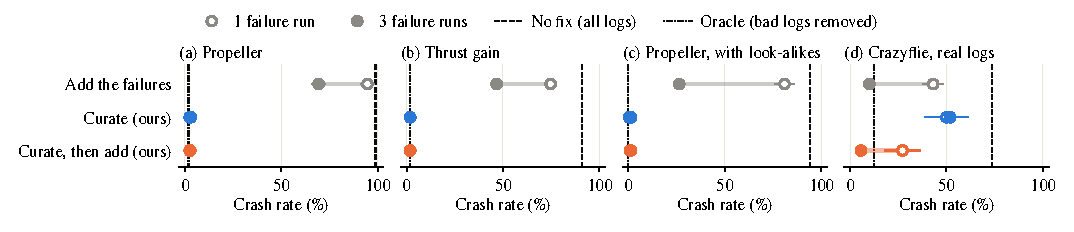
\includegraphics[width=\textwidth]{../figs/fig_failures.pdf}
\caption{Dives that crash (\%) after a fix using 1 (open) or 3 (filled) failure runs: add them ($W=20$), \method{} with the sign rule, or both. Mean $\pm$ s.e.\ over 5 seeds in (a), (b), (d), 3 in (c); where 1 and 3 runs coincide only the filled marker shows. Dashed: no fix; dotted: oracle. On the Crazyflie (d) curation alone fails; curating then adding three works.}
\label{fig:nfail}
\end{figure}

\subsection{How the scores rate the flights}\label{sec:scores}
Figure~\ref{fig:scores} shows one look-alike run. By training loss the faulty flights look like the rest, since the model fits the majority: worst-fit filtering's top 40 holds 22 of the 32 faulty flights and 12 of the 16 look-alikes, and the last faulty flight ranks 92nd of 95. \method{}'s score from one crash dive is positive for all 32 faulty flights, no look-alike and six other flights, so the sign rule removes 38.

\begin{figure}[t]
\centering
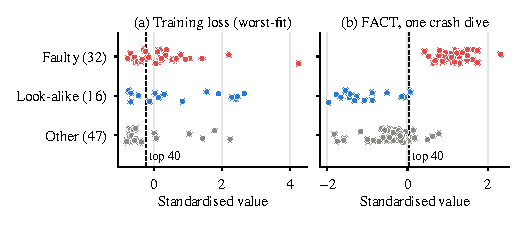
\includegraphics[width=0.75\textwidth]{../figs/fig_scores.pdf}
\caption{How each flight is rated on the look-alike benchmark (seed 1), one dot per flight; further right is more likely to be removed. (a) Training loss, used by worst-fit filtering. (b) \method{}'s score from one crash dive. Red: faulty; blue: correct look-alikes; grey: the rest.}
\label{fig:scores}
\end{figure}

\textbf{Count, checkpoint and rating.} A removal count matters only when too small: on the propeller fault the top 24 leave 8 bad flights and crash in 70\% of dives, while $k=32$ to 64 gives 1.7--3.3\% (5 seeds). Scoring at earlier checkpoints, or summing over all four as standard TracIn does, puts 31--32 bad flights in the top 40 on the propeller and gain faults. Rating a log by its top-scoring 2~s (the mean of its 200 highest sample scores, which need not be contiguous) instead of its mean changes little on the drone (Table~\ref{tab:major}: 2.2\% against 3.1\% on the propeller fault, 4.4\% against 1.9\% on the gain fault, with the sign rule's count), but the car needs it (Section~\ref{sec:car}).

\textbf{Without the gradient.} The gradient-free score uses the same crash dive, sign rule and retraining, but compares each sample's error with the dive's mean error instead of weighting the dive's states by the tangent kernel. On the quadrotor it does nearly as well (Table~\ref{tab:safe}). It removes 40--41 flights on the propeller benchmarks, 30--31 of them bad (AUROC 0.97--0.99), and exactly \method{}'s 32 on thrust gain, and it crashes in 1.4--3.9\% of dives against \method{}'s 0.9--3.1\%. It needs only forward passes, and on the propeller benchmark it keeps 49\% of the samples against 57\%, so the whole fix takes 6~s against \method{}'s 7~s. On these faults, then, what the crash supplies, labels of the deployed dynamics where the model is wrong, matters more than how the score weighs them, consistent with Proposition~\ref{prop:sign}, which covers this score ($k\equiv1$). The tangent kernel matters where the model cannot represent the plant: on the car, told the count, \method{} separates the bad logs from the look-alikes where the gradient-free score cannot (0.3\% against 20.3\%), and it finds 44--88 of a minority fault's 100 bad logs against 0--4 (Section~\ref{sec:car}). On the Crazyflie the two do the same (5.6\% and 5.3\%; Section~\ref{sec:cf}).

\subsection{Is it reweighting, extra training or less data?}\label{sec:reweight}

\begin{table}[t]
\caption{Other uses of the crash dive, and budget and removal-size controls: crash ($\pm$ s.e.) and reach (\%), 5 seeds (3 for look-alikes). Models take the full-data 2,640 updates unless marked ``fixed epochs'' (12 passes). $W$: crash-dive weight ($4{,}784$: half of every batch). Fine-tuning starts from the faulty model at a 10$\times$ smaller learning rate.}
\label{tab:reweight}
\centering\footnotesize
\setlength{\tabcolsep}{2.5pt}
\begin{tabular}{@{}lcccccc@{}}
\toprule
 & \multicolumn{2}{c}{Propeller} & \multicolumn{2}{c}{Thrust gain} & \multicolumn{2}{c}{Look-alike} \\
Fix (one crash dive) & Crash & Reach & Crash & Reach & Crash & Reach \\
\midrule
\method{}, sign rule, fixed epochs & \pmse{3.1}{1.2} & 61 & \pmse{1.9}{0.7} & 64 & \pmse{1.4}{0.8} & 79 \\
\quad unnormalised score, fixed epochs & \pmse{3.1}{0.8} & 60 & \pmse{3.6}{1.0} & 61 & \pmse{1.4}{0.8} & 69 \\
\quad 2,640 updates & \pmse{4.4}{0.7} & 52 & \pmse{3.1}{0.9} & 58 & \pmse{1.4}{0.0} & 78 \\
As many random flights, fixed epochs & \pmse{97.8}{0.7} & 34 & -- & & -- & \\
\quad 2,640 updates & \pmse{98.6}{0.0} & 35 & \pmse{91.7}{2.1} & 66 & \pmse{94.0}{2.6} & 37 \\
\midrule
Add, $W=20$, fixed epochs & \pmse{94.7}{3.6} & 36 & \pmse{74.7}{2.9} & 89 & \pmse{81.0}{5.2} & 49 \\
Add, $W=200$ & \pmse{89.2}{7.0} & 43 & -- & & -- & \\
Add, $W=2{,}000$ & \pmse{85.0}{7.4} & 49 & \pmse{64.4}{4.2} & 84 & \pmse{36.6}{12.3} & 70 \\
Add, balanced batches ($W=4{,}784$) & \pmse{79.4}{8.4} & 50 & \pmse{67.2}{5.0} & 85 & \pmse{28.2}{7.2} & 69 \\
Add, $W=20{,}000$ & \pmse{81.9}{11.5} & 44 & -- & & -- & \\
Fine-tune, half crash dive, half replay & \pmse{84.4}{14.5} & 39 & \pmse{83.1}{2.9} & 69 & \pmse{19.4}{6.4} & 65 \\
Fine-tune on the crash dive only & \pmse{70.6}{16.8} & 44 & -- & & -- & \\
Learning to reweight, crash dive as clean set & \pmse{2.8}{0.8} & 77 & \pmse{9.7}{1.7} & 86 & \pmse{2.3}{0.9} & 79 \\
\bottomrule
\end{tabular}
\end{table}

Table~\ref{tab:reweight} asks whether \method{}'s gain comes from its choice of logs, and whether the same crash dive could be used another way.

\textbf{Budget and removal size.} Removing as many random flights as the sign rule does leaves 92--99\% crashes, with the original schedule or with as many updates as the full-data model, while \method{} retrained for those 2,640 updates (about 18 passes over the kept data) gives 1.4--4.4\%: neither less data nor a different training budget explains the fix. Scoring without the normalisation removes nearly the same flights (31--32 of the 32 bad on the propeller fault, all 32 on the others, no look-alike) and gives 1.4--3.6\%.

\textbf{Heavier weights and fine-tuning.} On the propeller fault, raising the crash dive's weight from 20 up to balanced batches or $W=20{,}000$ lowers the crash rate only to 79--89\%, and fine-tuning the faulty model on the crash dive, with or without replayed logs, to 71--84\% (one seed of five responds to all of these, 4--61\%; the others stay at 76--100\%); on thrust gain they leave 64--83\%. The dive's 94 transitions correct the model along one trajectory, while new dives cross descent states the failure did not visit, where the faulty logs still dominate (Proposition~\ref{prop:add}). With look-alikes, correct flights cover those states and the faulty share is smaller (59\% of descent data against 67\%), and the same fixes do better (19--37\%) but stay far above \method{}'s 1.4\%.

\textbf{Learning to reweight.} With the crash dive as its clean set, learning to reweight is a second way to use the failure as a reference: it weights samples during training instead of removing logs. It matches \method{}'s crash rate on the propeller and look-alike benchmarks (2.8\% and 2.3\%), but crashes in 9.7\% on thrust gain, against 1.9\%. Its weights shut the bad logs out (thrust error about 5 standard units on faulty descent data), but on thrust gain, where the bad flights are wrong in every regime, it also fits correct descent data worse (1.1--2.0 units, against 0.4--0.8). It completes more dives safely on all three faults, with a smaller margin above the floor (Table~\ref{tab:safe}). The failure helps as a reference, not as data.

\textbf{Cost.} Table~\ref{tab:safe} gives the time of each complete fix on one CPU thread, from the logs and the crash record to a trained model (propeller benchmark; the other two take about as long, \ref{app:protocol}). An ordinary training takes 11~s and adding the crash dive 11~s. \method{} takes 7~s with its default schedule, of which 0.9~s is scoring, and 12~s with as many updates as the full-data model; with the gradient-free score the fix takes 6~s. Learning to reweight takes 31~s with the look-ahead of \citet{ren2018l2rw}, 27~s with one forward-mode product per batch, and 443~s with per-sample gradients, the form behind Table~\ref{tab:reweight}. Learning to reweight therefore needs substantially more computation in our implementation, and it returns a model rather than a dataset.

\subsection{Failures without a crash}\label{sec:sup}
Crashing a real drone is costly, so we also use runs that never crash. A supervisor watching the true state takes over the first time the drone could no longer stop above the floor with margin ($h<v^2/2a+0.1v+0.1$~m, with $h$ the height, $v$ the descent speed and $a$ the spare thrust) and commands full thrust and level attitude. It saves every dive, about 0.7~s before impact. Scored from the first supervised run through the takeover, the sign rule finds all 32 bad flights on every seed, removes no look-alike, and the planner crashes in 1.4--3.1\% of dives (Table~\ref{tab:major}). The takeover matters: it is full thrust in fast descent, exactly where the propeller fault shows, while before it the faulty model brakes late at or below hover thrust, so that part alone finds only 18--31 of the 32 bad flights and crashes in \pmse{75.3}{10.0}\% of dives. A failure need not crash, but must record the attempt to recover.

\subsection{What the reference must cover}\label{sec:ref}

\begin{table}[t]
\caption{The reference \method{} scores against, each with the crash dive's number of transitions (93--99) and labelled by the plant. Desc.: share of the reference's transitions descending along the rotor axis faster than 1~m/s, where the propeller faults act (range over the three benchmarks). Error: the faulty model's mean squared error on the reference (normalised units). Found: bad flights removed (of 32) / flights removed (of 95), mean over seeds. Crash: dives that crash (\%, $\pm$ s.e.), 5 seeds (3 for look-alikes); the crash-dive row is Table~\ref{tab:safe}'s \method{} row.}
\label{tab:ref}
\centering\footnotesize
\setlength{\tabcolsep}{2pt}
\begin{tabular}{@{}lcccccccccc@{}}
\toprule
 & & \multicolumn{3}{c}{Propeller} & \multicolumn{3}{c}{Thrust gain} & \multicolumn{3}{c}{Look-alike} \\
Reference & Desc. & Error & Found & Crash & Error & Found & Crash & Error & Found & Crash \\
\midrule
Crash dive & 0.34--0.39 & 9.0 & 31.8/35.2 & \pmse{3.1}{1.2} & 7.4 & 32/32 & \pmse{1.9}{0.9} & 6.1 & 32/43 & \pmse{0.9}{0.5} \\
Expert dive & 0.32--0.38 & 3.3 & 31.6/33.8 & \pmse{4.4}{0.7} & 3.7 & 32/32 & \pmse{1.9}{0.9} & 2.4 & 32/34.3 & \pmse{0.9}{0.5} \\
Routine flight & 0.15--0.18 & 3.3 & 32/38 & \pmse{3.3}{1.3} & 4.2 & 32/32 & \pmse{1.9}{0.9} & 2.2 & 32/47.3 & \pmse{2.8}{0.8} \\
Hover & 0.00 & 0.01 & 21.4/38.6 & \pmse{94.7}{0.9} & 1.2 & 32/32 & \pmse{1.9}{0.9} & 0.01 & 21.7/40 & \pmse{92.1}{1.2} \\
\bottomrule
\end{tabular}
\end{table}

Proposition~\ref{prop:ident} needs only correctly labelled data from the deployed robot in the faulty regime, and a failure is one such record. To separate what the failure contributes as a failure from what it contributes as coverage of that regime, Table~\ref{tab:ref} scores against four records of the same length: the crash dive; an expert dive, the crash dive's start and goal flown for as long by a planner that uses the plant as its model (standing in for a pilot or a conservative controller); a routine flight, the faulty model's first flight down the hangar that stops short of the end wall without crashing, thinned to the same number of transitions; and the faulty model holding its start position. The expert dive and the routine flight work about as well as the crash, finding all or nearly all 32 bad flights (crashes in 0.9--4.4\% of dives, against 0.9--3.1\%); the routine flight, with less than half the descent, removes more correct flights with the look-alikes (15 on average, against 11). Hover has no descent along the rotor axis, and on the propeller faults the faulty model already fits it (error 0.01, against 6.1--9.0 on the crash dive): it finds 21--22 of the 32 bad flights, and the planner crashes nearly as often as without a fix (92--95\% against 94--99\%). On thrust gain, a fault that acts in every regime, the faulty model is wrong in hover too, and hover finds all 32 (1.9\%). What \method{} needs is a correctly labelled record of the regime where the logs are wrong. A failure is the record the planner produces there by itself, without anyone knowing which regime that is; an ordinary flight that covers the regime, by design or incidentally as the routine flight does here, serves as well, and the faulty model's error on a candidate reference shows whether it reaches the fault.

\subsection{Robustness}\label{sec:robust}

\begin{table}[t]
\caption{Propeller benchmark under other conditions: dives that crash (\%), 5 seeds ($\pm$ s.e.\ for \method{}). Top: another plant flies the failure run and judges every fix. Bottom: degraded failure records; Found: bad flights removed (of 32). Right: a milder fault (+35\%) with 16 look-alikes (37\% crashes unfixed). Under the mismatch even the oracle crashes in 22\%: what remains is plant mismatch, not curation. The default row's \method{} is 3.1 here and in Table~\ref{tab:major}, and 21.9 against 22.2 under the mismatch, because the two use the same sign rule and the oracle's crashes are the mismatch's. $^\ast$Plant fit on 32 held-out flights; the logs are the other 63 (20 faulty), so no plant data reach the planner's model.}
\label{tab:plants}
\centering\footnotesize
\setlength{\tabcolsep}{4pt}
\begin{tabular}{@{}lcccc@{}}
\toprule
Plant & Unfixed & Add crash & \method{} & Oracle \\
\midrule
Default (Table~\ref{tab:major}) & 98.9 & 94.7 & 3.1$\pm$1.2 & 1.9 \\
MLP 3$\times$256 tanh & 98.9 & 93.1 & 1.4$\pm$0.4 & 1.4 \\
MLP 2$\times$64, 70\% of flights & 98.3 & 91.4 & 2.2$\pm$0.7 & 1.7 \\
Boosted trees & 98.9 & 87.2 & 1.4$\pm$0.8 & 1.7 \\
Default + mismatch & 98.1 & 95.6 & 21.9$\pm$1.4 & 22.2 \\
Cross-fitted$^\ast$ & 93.9 & 54.7 & 1.9$\pm$0.6 & 1.9 \\
\midrule
 & \multicolumn{2}{c}{Benchmark} & \multicolumn{2}{c}{+35\%, look-alikes} \\
Failure record & Crashes & Found & Crashes & Found \\
\midrule
Crash, as simulated & 3.1$\pm$1.2 & 31--32 & 5.0$\pm$2.3 & 30--32 \\
State noise $\times$1 & 3.1$\pm$1.2 & 31--32 & 4.7$\pm$2.4 & 30--32 \\
\quad $\times$3 & 3.1$\pm$1.2 & 31--32 & 5.8$\pm$2.8 & 30--32 \\
First 75\% of the run & 3.1$\pm$0.5 & 31--32 & 3.3$\pm$1.4 & 32 \\
First 50\% & 62.8$\pm$15.7 & 15--31 & 16.7$\pm$3.3 & 19--25 \\
Supervisor, margin 0.1~m & 3.1$\pm$0.7 & 32 & 3.1$\pm$0.5 & 31 \\
\quad 0.5~m & 3.9$\pm$0.3 & 31--32 & 3.3$\pm$1.2 & 31 \\
\quad 1.0~m & 2.2$\pm$0.6 & 32 & 1.9$\pm$0.6 & 31 \\
\quad 0.3~s reaction & 2.8$\pm$0.6 & 32 & 1.9$\pm$0.3 & 31 \\
\quad 0.5~m + noise $\times$1 & 3.9$\pm$0.3 & 31--32 & 1.4$\pm$0.0 & 31 \\
\bottomrule
\end{tabular}
\end{table}

\textbf{Other plants.} With the plant that flies the failure run and judges every fix replaced by a wider tanh MLP, a smaller MLP fit on 70\% of the flights, or gradient-boosted trees, \method{} removes 31--32 of the 32 bad flights and stays within 0.5 points of the oracle, while adding the crash leaves 87--93\% (Table~\ref{tab:plants}, top). These plants fit the logs as well as the default plant ($R^2$ 0.86--0.98 per axis) but differ from it by 0.17--0.29~m/s$^2$ on average. The mismatch plant adds to the default one a 30~ms motor lag, 1~m/s$^2$ gusts, 5\% less thrust than commanded and a state estimate with correlated noise (2~cm, 0.05~m/s, 0.6$^\circ$, 0.05~rad/s), which the planner and the failure record see. On every one of these plants \method{} removes 31--32 of the 32 bad flights (33--36 in all). In a cross-fitted test the plant is fit on a third of the flights, every third by axial descent within each day, and the planner's logs are the other 63 flights, 20 of them faulty (64\% of the descent data), so the data that define the plant never reach the planner's model. The plant predicts the unseen flights with $R^2$ 0.84--0.96 per axis; \method{} removes all 20 bad flights (20--38 in all) and matches the oracle on every seed (1.9\%), while adding the crash leaves 55\%. Under the mismatch, the oracle and \method{} both crash in 22\%: curation removes wrong logs but cannot supply dynamics that no log records.

\textbf{Imperfect failure records.} Logging the run from the noisy state estimate, or from three times its noise, changes nothing (Table~\ref{tab:plants}, bottom). Neither does a supervisor that takes over earlier (0.5 or 1.0~m margin) or reacts in 0.3~s, nor a noisy, supervised run with a milder fault and look-alikes. State noise and earlier or slower takeovers leave 1.4--5.8\% crashes. With its first half only, the record misses most of the fast descent where the fault shows, finds 15--31 bad flights and leaves 63\% crashes on average (17\% with the milder fault).

\begin{table}[t]
\caption{Robustness on the propeller fault, one factor at a time from the benchmark (+50\% thrust, 32 bad flights); sign rule from one crash dive, 3 seeds (5 for +20\%, 44 bad and 32 look-alikes). Bad: share of descent data from bad flights. Removed: flights removed of 95 (bad / look-alikes). Crash rates (\%): unfixed, \method{} ($\pm$ s.e.), oracle.}
\label{tab:sweep}
\centering\footnotesize
\setlength{\tabcolsep}{4pt}
\begin{tabular}{@{}lccccc@{}}
\toprule
Setting & Bad & Removed & Unfixed & \method{} & Oracle \\
\midrule
Benchmark & 67\% & 33--36 (32 / 0) & 98.6 & 3.7$\pm$1.7 & 0.9 \\
Thrust +20\% & 67\% & 39--55 (29--32 / 0) & 10.3 & 3.3$\pm$0.8 & 1.9 \\
\quad +35\% & 67\% & 33--37 (31--32 / 0) & 86.6 & 3.7$\pm$0.5 & 0.9 \\
\quad +80\% & 67\% & 33--35 (32 / 0) & 100.0 & 4.2$\pm$1.6 & 0.9 \\
Bad flights 12 & 32\% & 23--44 (12 / 0) & 43.1 & 1.4$\pm$0.8 & 0.5 \\
\quad 20 & 50\% & 27--31 (20 / 0) & 92.6 & 0.5$\pm$0.5 & 0.9 \\
\quad 44 & 80\% & 46--59 (42--44 / 0) & 98.9 & 4.7$\pm$3.1 & 3.1 \\
Plus look-alikes 8 & 61\% & 34--39 (32 / 0) & 95.8 & 1.9$\pm$1.2 & 0.0 \\
\quad 16 & 56\% & 40--60 (32 / 1--3) & 90.3 & 0.9$\pm$0.5 & 2.3 \\
\quad 32 & 49\% & 34--52 (27--30 / 0--11) & 71.1 & 1.9$\pm$0.7 & 0.6 \\
\bottomrule
\end{tabular}
\end{table}

\textbf{Severity, faulty share and look-alikes.} Table~\ref{tab:sweep} varies the propeller benchmark one factor at a time (its first three seeds, hence 3.7 rather than 3.1 for the benchmark row). From +20\% to +80\% thrust, 12 to 44 bad flights (32--80\% of the descent data) and up to 32 look-alikes, \method{} stays within 3.3 points of the oracle (mean crash rates 0.5--4.7\%, worst seed 17\%), against 43--100\% unfixed except under the mildest fault. At +20\% thrust the crash run carries a smaller error, yet the sign rule still finds 29--32 of the 32 bad flights. With 44 bad flights (80\% of the descent data), one seed of five misses two and crashes in 17\%, the worst single seed of the study; the others crash in 0--4\%. With 32 correct look-alikes the score separates less cleanly (AUROC 0.80--0.99): the sign rule misses up to five bad flights and removes up to 11 look-alikes, yet no seed crashes in more than 4.2\% of dives, and the planner reaches the goal as often as the oracle's (56--96\% against 57--97\% of dives in these three settings).

\subsection{A fault that starts mid-flight}\label{sec:local}

\begin{table}[t]
\caption{Fault that starts mid-flight: +50\% thrust in descent from 25--50\% into each of the 44 most-descending flights (63\% of descent data faulty; 5 seeds). Fail.: crash runs used (the second from the curated model). Removed: faulty / correct descent data (\%). Kept: data kept (\%).}
\label{tab:local}
\centering\footnotesize
\setlength{\tabcolsep}{3pt}
\begin{tabular}{@{}lcccc@{}}
\toprule
Rule & Fail. & Crash (\%) & Removed & Kept \\
\midrule
Unfixed & -- & 96.7$\pm$0.3 & -- & 100 \\
\method{}, flights & 1 & 37.5$\pm$17.8 & 70--98 / 27--43 & 42--52 \\
\method{}, flights & 2 & 5.3$\pm$2.6 & 100 / 47--75 & 25--33 \\
\method{}, 2-s windows & 1 & 60.6$\pm$11.7 & 93--98 / 3--5 & 47--49 \\
Oracle, flights & -- & 3.1$\pm$0.7 & 100 / 46 & 47 \\
Oracle, 2-s windows & -- & 14.7$\pm$2.2 & 99 / 2 & 68 \\
Oracle, samples & -- & 1.1$\pm$0.3 & 100 / 0 & 68 \\
\bottomrule
\end{tabular}
\end{table}

So far a bad log is wrong from start to end. When the propeller fault instead starts 25--50\% into each of the 44 most-descending flights, so that 21\% of their descent data is still correct, one failure is not enough (Table~\ref{tab:local}): the flight mean mixes the two parts, the sign rule finds 37--43 of the 44 flights, two of five seeds crash in about 80\% of dives, and the planner crashes in \pmse{37.5}{17.8}\% of dives on average (unfixed 97\%). Rating 2-s windows locates the fault (AUROC 0.96--0.99 over windows with descent) but still crashes in 61\% (single samples: 36\%): a window has too few samples to average out label noise where the faulty model sits between the two groups (Proposition~\ref{prop:agg}), and the planner is sensitive to what is left, since even removing exactly the mostly-faulty windows crashes in 15\%. A second failure, a crash of the curated model, fixes the flight rule: it finds all 44 flights on every seed and crashes in \pmse{5.3}{2.6}\% (flight oracle 3.1\%). The price is data: \method{} removes the faulty flights whole, plus 14--26 correct ones, and keeps 25--33\% of the data against 68\% for an oracle that removes only the faulty samples. \method{} works on whole logs: it finds the logs a fault enters partway but cannot separate their parts.

\subsection{A car whose model cannot represent the plant}\label{sec:car}

\begin{table}[t]
\caption{MuJoCo car, most fast icy logs faulty: runs that crash (\%, 5 seeds); bad logs (of 300) / look-alikes (of 100) removed.}
\label{tab:mj}
\centering\footnotesize
\setlength{\tabcolsep}{4pt}
\begin{tabular}{@{}lccc@{}}
\toprule
Fix & Fail. & Crash & Bad / look. \\
\midrule
None (all logs) & 0 & \pmse{39.7}{3.7} & -- \\
Oracle & -- & \pmse{0.0}{0.0} & 300 / 0 \\
Huber loss & 0 & \pmse{41.7}{5.2} & -- \\
L1 loss & 0 & \pmse{77.8}{2.8} & -- \\
Remove 360 worst-fit & 0 & \pmse{48.1}{7.6} & 0 / 22--32 \\
Drop 360 most crash-like & 0$^\S$ & \pmse{3.3}{2.3} & 233 / 68 \\
Drop all fast data on ice & 0$^\S$ & \pmse{21.1}{12.1} & -- \\
Add crash runs, $W=20$ & 1 & \pmse{26.7}{6.7} & -- \\
 & 3 & \pmse{10.3}{4.6} & -- \\
\textbf{\method{}}, sign count$^\dagger$ & 1 & \pmse{1.4}{1.1} & 300 / 100$^\ast$ \\
 & 3 & \pmse{0.0}{0.0} & 300 / 100$^\ast$ \\
Gradient-free, sign count$^\dagger$ & 1 & \pmse{0.8}{0.6} & 300 / 100$^\ast$ \\
\method{}, remove 360 & 3 & \pmse{0.3}{0.3} & 283--300 / 50--60 \\
Gradient-free, remove 360 & 3 & \pmse{20.3}{15.9} & 229--288 / 63--100 \\
\bottomrule
\end{tabular}\\[2pt]
\footnotesize $^\dagger$As many logs as have a positive mean score, ranked by their top-scoring 2~s. $^\S$Uses where crashes happen. $^\ast$1,338--1,713 of 2,910 removed.
\end{table}

A MuSHR car~\citep{srinivasa2019mushr} in MuJoCo~\citep{todorov2012mujoco} drives an L-shaped corridor whose corner is icy (friction 0.2); the learned model predicts 50~ms body-frame state changes, and we drive 24 runs from each of three entry conditions (test, late entry, entry at the ice edge). In the majority fault, 300 fast route runs recorded on a dry day make up 65\% of the fast data over the ice, alongside 100 correct fast icy runs (look-alikes) and about 2,500 short exploration logs. The 300 faulty route runs were recorded with dry-road friction, so they are wrong only over the ice. The fault crashes the planner in 40\% of runs, and robust losses and worst-fit filtering do no better (Table~\ref{tab:mj}).

Here we depart from the sign rule. The failure target is the last 2~s before contact, and logs are ranked by their top-scoring 2~s (the mean of their 40 highest sample scores), since the mean puts only 0--32 of the 300 bad logs in the top 360; the sign rule only sets how many to remove, the number of logs with a positive mean score (about 1,500 of 2,910). This fixes the planner from one crash run (1.4\%), but not selectively. The car's model cannot represent the ice even with correct logs: without the faulty logs it still keeps 72--81\% of the error on the crash runs, against about 1\% for the drone. Assumption (ii) therefore fails, every score shifts up, and \method{} removes about half of all logs, route runs and look-alikes included: a regime filter, which the gradient-free score matches (0.8\%). The logs removed are the top-ranked ones: all 410 route runs, so all 100 look-alikes, and 1,000--1,200 exploration logs. The 1,300--1,800 samples of fast driving on the ice left in the kept exploration logs are what keep the planner off the wall. Told the count, \method{} from three runs removes 283--300 of the bad logs and about half the look-alikes (0.3\%), where the gradient-free score cannot tell them apart (20.3\%); but dropping the 360 logs with the most fast driving on the ice does nearly as well (3.3\%).

On a minority car fault (100 bad logs) the gradient-free score finds 0--4 of the bad logs against 44--88 for TracIn: where the model cannot represent the plant, correct logs near the failure have errors like the bad ones, and the tangent kernel, which weighs how training on a log changes the model at the failure states, separates them.

\subsection{A fault in real logs: Crazyflie battery sag}\label{sec:cf}

\begin{table}[t]
\caption{Crazyflie battery sag (real logs): crash and reach (\%, 5 seeds). The battery voltage is logged but withheld from the planner's model. The oracle keeps only the low-voltage flights, the correct historical subset; the last row adds the same three crash dives to it.}
\label{tab:cf}
\centering\footnotesize
\setlength{\tabcolsep}{4pt}
\begin{tabular}{@{}lccc@{}}
\toprule
Fix & Fail. & Crash & Reach \\
\midrule
None (all flights) & 0 & \pmse{73.6}{3.4} & 24 \\
Oracle (low voltage) & -- & \pmse{12.5}{5.2} & 80 \\
Huber loss & 0 & \pmse{66.7}{2.8} & 35 \\
L1 loss & 0 & \pmse{77.8}{3.1} & 30 \\
Remove 76 worst-fit & 0 & \pmse{78.9}{4.9} & 29 \\
Remove 76 random & 0 & \pmse{70.9}{6.0} & 38 \\
Drop 76 most crash-like & 0$^\S$ & \pmse{80.3}{7.3} & 26 \\
Add crash dives & 1 & \pmse{43.1}{5.5} & 59 \\
 & 3 & \pmse{10.0}{3.0} & 87 \\
Learning to reweight & 1 & \pmse{49.4}{14.9} & 50 \\
 & 3 & \pmse{19.7}{6.1} & 77 \\
Learning to reweight + add & 1 & \pmse{24.2}{14.9} & 74 \\
 & 3 & \pmse{10.0}{5.4} & 91 \\
\method{}, sign rule & 1 & \pmse{50.0}{11.5} & 49 \\
 & 3 & \pmse{51.9}{5.5} & 49 \\
\method{}, sign rule + add & 1 & \pmse{27.2}{9.2} & 71 \\
 & 3 & \textbf{\pmse{5.6}{1.8}} & 92 \\
Gradient-free, sign + add & 3 & \pmse{5.3}{1.8} & 94 \\
Oracle + add & 3 & \pmse{1.7}{0.8} & 96 \\
\bottomrule
\end{tabular}\\[2pt]
\footnotesize $^\S$Uses where crashes happen.
\end{table}

NanoBench~\citep{ullah2026nanobench} logs flights of a Crazyflie 2.1 with motor commands and battery voltage; we use the 105 of its 107 public recordings that keep at least 2~s of airborne data (\ref{app:protocol}); at low voltage the same command gives less thrust. The voltage is recorded in every log but deliberately withheld from the planner's model, as a stand-in for causes that are not logged, such as propeller wear; with the voltage as an input there would be nothing to curate (Section~\ref{sec:practice}). The plant sees the voltage and flies at 3.1~V, so the 76 flights flown at a median of 3.35~V or more (73\% of the data) are consistently wrong for this battery. Every model takes equal gradient steps. Every fix without failures crashes in 67--80\% of dives, against 12.5\% for the low-battery flights alone (still above 3.1~V; Table~\ref{tab:cf}). Unlike on the built faults, curation alone fails, from one crash or three (50--52\%): the crash's error is as large sideways as vertical, so the score also reflects how much a flight resembles the dive (assumption (ii) fails), and the fault is a continuum (AUROC 0.35--0.63), so \method{} does not reliably find the faulty flights here. Learning to reweight does better from three crashes (19.7\%). Three crashes help mostly as data: adding them alone gives 10.0\%, and curating with them first gives 5.6\%, the same as the gradient-free score curated and added the same way (5.3\%). This experiment therefore supports curating and then adding, not the gradient score. Given the same three crashes, the oracle's correct historical flights crash in 1.7\%. The smaller differences are within noise. Paired over seeds, \method{} plus adding minus adding alone is $-4.4$ points (95\% CI $-9.8$ to $0.9$; lower on four seeds, tied on one); minus reweighting and adding, $-4.4$ ($-16.0$ to $7.1$; reweighting's worst seed crashes in 29\% against 11\%); minus the gradient-free score, $+0.3$ ($-4.8$ to $5.4$); and minus the oracle with the crashes added, $+3.9$ ($-3.3$ to $11.0$). With the plant fit on a held-out third of flights, curating and adding is again below adding alone (26\% against 36\%; oracle 52\%).

\subsection{Where failures are not needed}\label{sec:minority}
Our claim is limited to consistent faults that dominate a regime. With 12 propeller-faulty flights (a minority) among 12 correct look-alikes and 12 harmless noisy flights, an L1 loss crashes in 2\% of dives and removing the 20 worst-fit flights in 5\%, against 1.4\% for \method{} (5 seeds). With the motor log 100~ms late on the 32 most-descending flights, a majority but inconsistent fault, the lagged logs fit poorly and worst-fit removal fixes the model (4\%, seed 1); \method{} matches it only when each log is rated by its top-scoring 2~s of samples (2.8\%, against 31\% with the mean).

\section{Discussion}\label{sec:discussion}

\subsection{Where the analysis holds and where it fails}\label{sec:assumptions}

\begin{table}[p]
\caption{Each condition of the analysis (Section~\ref{sec:analysis}), where it holds and fails in our experiments, and what \method{} does where it fails. Crash rates in \%.}
\label{tab:assume}
\centering\footnotesize
\renewcommand{\arraystretch}{1.15}
\setlength{\tabcolsep}{3pt}
\begin{tabular}{@{}L{0.19\textwidth}L{0.21\textwidth}L{0.24\textwidth}L{0.3\textwidth}@{}}
\toprule
Condition & Holds & Fails & What happens \\
\midrule
A consistent fault that dominates a regime (Section~\ref{sec:problem}) & Every quadrotor and car majority fault; the Crazyflie battery fault & A minority fault; a motor log 100~ms late (inconsistent) & Failures are not needed: an L1 loss (2) or worst-fit removal (5; 4 for the lag) already works (Section~\ref{sec:minority}) \\
(ii) The failure's error comes from the fault alone & Quadrotor: without the faulty logs about 1\% of the crash runs' error remains & Car: 72--81\% remains; Crazyflie: the crash's error is as large sideways as vertical & Car: a regime filter that removes about half of all logs (1.4); Crazyflie: curation alone fails (50--52), and the crashes added do most of the work (10.0 added alone, 5.6 curated and added) \\
(iii) Two groups, each fault of fixed direction & The built faults & Crazyflie: a voltage continuum, not two groups (AUROC 0.35--0.63) & As above \\
(iv) A nonnegative scalar kernel & After averaging over the failure and a flight: 88\% of bad flights meet the margin condition & Pair by pair (scalar part negative for 1--36\% of pairs); at +20\% thrust the margin shrinks & The sign rule still finds 29--32 of 32 at +20\% (Section~\ref{sec:margin}); the gradient-free score, whose kernel meets (iv), crashes in 1.4--3.9 (Section~\ref{sec:scores}) \\
(v) Normalisation keeps the sign & Not checked directly & -- & Without the normalisation the score removes nearly the same flights (1.4--3.6) \\
Whole logs are faulty (Proposition~\ref{prop:agg}) & The built faults & A fault that starts mid-flight & One failure: 37.5; a second failure: 5.3, keeping 25--33\% of the data (Section~\ref{sec:local}) \\
The reference records the faulty regime & A crash, or a takeover with the recovery; an expert dive or a routine flight through the regime & The first half of the run; the supervised run before the takeover; hover & 63, 75.3 and 92--95 (Sections~\ref{sec:sup}, \ref{sec:ref} and~\ref{sec:robust}) \\
The logs record the plant up to the fault & Other learned plants, one fit on flights the planner never saw (within 0.5 points of the oracle) & Unlogged motor lag, gusts, thrust deficit and estimation noise & \method{} and the oracle both crash in 22: curation cannot supply missing dynamics \\
\bottomrule
\end{tabular}
\end{table}

Table~\ref{tab:assume} collects, for each condition of Section~\ref{sec:analysis}, the experiments where it holds and fails. Two patterns stand out. First, \method{} degrades gracefully when a condition is only weakened: a shrinking margin under a mild fault, look-alikes that blur the separation, and noisy or earlier failure records all leave crash rates within a few points of the oracle. Second, it stops working as curation when a condition fails outright: when the failure's error does not come from the fault, when a log is only partly faulty, or when the record misses the faulty regime. Most of these cases have a remedy within the same framework: adding the failures as data (Crazyflie, where they do most of the work), a second failure (mid-flight fault), or a record that includes the recovery (supervised runs). The car has none: \method{} still fixes the planner there, but as a regime filter that a crude location rule nearly matches.

\subsection{Using \method{} in practice}\label{sec:practice}

The experiments suggest the following checks for a practitioner. They are drawn from our simulated benchmarks and have not been validated on hardware.
\begin{itemize}
\item \textbf{Rule out a minority or inconsistent fault first.} If the logs a failure implicates fit the model poorly, robust losses or worst-fit removal are cheaper and work (Section~\ref{sec:minority}). \method{} is for logs that fit well and are wrong.
\item \textbf{Record the recovery, not only the crash.} A supervisor's takeover is as useful as a crash, provided the record includes it (Section~\ref{sec:sup}); a record that stops before the regime where the fault shows is not (Table~\ref{tab:plants}). A correctly labelled ordinary flight that covers that regime serves as the reference, and a record on which the model already fits well, such as hover on the propeller faults, does not (Section~\ref{sec:ref}).
\item \textbf{Read the removed set.} \method{} returns the logs it removes. On the quadrotor these were 32--47 flights, including 31--32 of the 32 faulty ones. When it removes a large share of all logs, as on the car, it is acting as a regime filter, a sign that the model cannot represent the plant there. Retraining without the removed logs and measuring the error left on the failure distinguishes the two: in our runs, removing the faulty logs left about 1\% of the drone's error on the crash runs and 72--81\% of the car's.
\item \textbf{If the curated model fails again, use that failure.} A second failure fixed the fault that starts mid-flight (Section~\ref{sec:local}).
\item \textbf{If the cause of the fault is logged, add it as a model input} rather than curating around it, as the battery voltage could be on the Crazyflie.
\item \textbf{Choose between \method{} and learning to reweight by what is needed.} With the failure as its clean set, reweighting completed more dives safely on all three faults (76--83\% against 60--79\%), with a smaller margin above the floor, but crashed more on the thrust-gain fault and needs more computation. \method{} costs one scoring pass and one training, and returns an explicit dataset that can be inspected, versioned and reused by any training pipeline.
\end{itemize}

\subsection{Limitations}\label{sec:limits}
All closed-loop results are simulated. The quadrotor plants are fit to real flight logs and the battery fault comes from real logs, but no curated model has flown on hardware, and the mismatch experiment shows that unmodelled effects set a floor that curation cannot lower. The drone and car faults are built by us; the battery fault shows the problem is real, but its cause is withheld rather than unknown. \method{} curates whole logs and needs a second failure when a fault enters a log partway. It needs a reference that covers the regime where the model is wrong. Failures can expose that regime without prior identification; other trajectories also work when they cover it. Failures are costly on a real robot; a supervisor's takeover reduces but does not remove that cost. On the car a crude location rule nearly matches it.

\section{Conclusion}\label{sec:conclusion}
When a consistent fault covers most of the logs in a regime, the logs alone cannot reliably identify which group matches the deployed dynamics, and a few failures added at a fixed weight are outvoted. Used as a reference, one failure run finds the wrong logs on the quadrotor and fixes planners that every failure-free fix leaves crashing; on the real-log battery fault, a continuum, curation alone fails and three failures help mainly as added data. What the failure contributes is coverage: a correctly labelled routine or expert flight through the faulty regime serves as well, hover does not suffice for the descent-specific propeller faults, and on the quadrotor a score that compares errors without the gradient does nearly as well. Learning to reweight with the failure as its clean set reaches comparable crash rates on two quadrotor benchmarks and completes more dives safely on all three, with a smaller margin above the floor; \method{} crashes less on the third, needs less computation and produces an explicit curated dataset. The analysis explains these results at the level of whole logs, and the conditions that fail mark where \method{} stops: minority faults need no failures, models that cannot represent the plant turn curation into a regime filter, and partly faulty logs need a second failure. These results come from controlled simulations built from real flight logs, not from deployment. Next is hardware, with a supervisor's takeover as the failure, and separating a log's correct part from its faulty part.

\section*{CRediT authorship contribution statement}
\textbf{Apurba Bose:} Conceptualization, Methodology, Software, Formal analysis, Investigation, Visualization, Writing -- original draft. \textbf{Soovadeep Bakshi:} Conceptualization, Methodology, Software, Formal analysis, Investigation, Visualization, Writing -- original draft. \textbf{Jiachen Li:} Methodology, Investigation, Writing -- review \& editing. \textbf{Dongmei Chen:} Supervision, Resources, Writing -- review \& editing.

\section*{Declaration of competing interest}
The authors declare that they have no known competing financial interests or personal relationships that could have appeared to influence the work reported in this paper.

\section*{Funding}
This research did not receive any specific grant from funding agencies in the public, commercial, or not-for-profit sectors.

\section*{Data availability}
The NeuroBEM~\citep{bauersfeld2021neurobem} and NanoBench~\citep{ullah2026nanobench} datasets are publicly available. The code, the flight splits and fault construction, the baseline settings, the per-seed result files behind every number in this paper and a script that recomputes those numbers are available at \url{https://github.com/soovadeep/few-crash-curation}.

\section*{Declaration of generative AI and AI-assisted technologies in the manuscript preparation process}
During the preparation of this work the authors used Claude (Anthropic) in order to search the literature, to write and run the experiment code, and to draft and edit the text. After using this tool, the authors reviewed and edited the content as needed and take full responsibility for the content of the published article. A script in the code repository recomputes every number in this paper from the stored result files.

\bibliographystyle{elsarticle-num-names}
\bibliography{../refs}

\appendix

\section{Proofs}\label{app:proofs}

\textbf{Proposition~\ref{prop:sign}.} Say $f^\star=g_2$. Then $e_t=\rho\Delta(x_t)$, and in expectation a faulty sample has $e_i=-(1-\rho)\Delta(x_i)$ and a correct one $e_i=\rho\Delta(x_i)$. So $\E\phi_i=\rho(1-\rho)\sum_t k\langle\Delta(x_t),\Delta(x_i)\rangle>0$ for a faulty sample and $-\rho^2\sum_t k\langle\Delta(x_t),\Delta(x_i)\rangle<0$ for a correct one. The case $f^\star=g_1$ is symmetric.

\textbf{Normalisation.} The expectation of a ratio need not have the sign of the ratio of expectations: a scalar residual with mean $0.5$ and noise $+3$ or $-1$ with probabilities $\frac14$ and $\frac34$ has $\E[e/|e|]=-\frac12$, so its normalised score has the opposite expected sign to its unnormalised one. Proposition~\ref{prop:norm} rules this out with symmetric noise in two or more dimensions; in one dimension symmetry is not enough, since mean $0.5$ and noise uniform on $[-3,-2]\cup[2,3]$ give $\E[e/|e|]=0$.

\textbf{Proposition~\ref{prop:norm}.} In this setting $\hat f$ and the failure residuals $e_t$ are fixed by (i) and (ii), so $a_i=\sum_tk(x_t,x_i)e_t$ does not depend on sample $i$'s label noise; only $e_i$ does. Then $\phi_i=-\langle a_i,e_i\rangle$ and, since $J_iJ_i^\top=c_iI$, $\|J_i^\top e_i\|=\sqrt{e_i^\top J_iJ_i^\top e_i}=\sqrt{c_i}\|e_i\|$, so $\tilde\phi_i=-\langle a_i,e_i/\|e_i\|\rangle/\sqrt{c_i}$. Write $e_i=m+\varepsilon$ with $m=\E e_i\ne0$, $u=m/\|m\|$, $s=\langle\varepsilon,u\rangle$ and $r$ the norm of the rest of $\varepsilon$. Negating the part of $\varepsilon$ orthogonal to $u$ leaves its distribution unchanged, so $\E[e_i/\|e_i\|]$ is parallel to $u$, with component $\E\,h_r(\|m\|+s)$, $h_r(z)=z/\sqrt{z^2+r^2}$. Given $r$, $s$ is symmetric about zero, and $h_r$ is odd and increasing, so $h_r(\|m\|+s)+h_r(\|m\|-s)\ge0$, strictly when $r>0$, which holds almost surely for outputs of two or more dimensions. Hence $\E[e_i/\|e_i\|]=\kappa u$ with $\kappa>0$, and $\E\tilde\phi_i=-\kappa\langle a_i,m\rangle/(\sqrt{c_i}\|m\|)$ has the sign of $\E\phi_i=-\langle a_i,m\rangle$.

\textbf{Proposition~\ref{prop:agg}.} Take $\mu>0$; the other case is symmetric. Let $S=\sum_j(c_j-\E c_j)$, so the mean score is at most zero only if $S\le-n\mu$. Split the indices into the $\tau$ classes $j\bmod\tau$, with $n_r$ elements and sums $S_r$. By $\tau$-dependence the terms within a class are jointly independent, so $\E e^{-\lambda\tau S_r}\le e^{\lambda^2\tau^2\sigma^2n_r/2}$, and the generalised H\"older inequality gives
\begin{equation*}
\E e^{-\lambda S}=\E\prod_re^{-\lambda S_r}\le\prod_r\big(\E e^{-\lambda\tau S_r}\big)^{1/\tau}\le e^{\lambda^2\tau\sigma^2n/2}.
\end{equation*}
 Markov's inequality with $\lambda=\mu/(\sigma^2\tau)$ gives
\begin{equation*}
P(S\le-n\mu)\le e^{-\lambda n\mu+\lambda^2\sigma^2n\tau/2}=e^{-n\mu^2/(2\tau\sigma^2)}.
\end{equation*}
 A cosine lies in $[-1,1]$, so it is $1$-sub-Gaussian by Hoeffding's lemma. The bound over logs is a union bound. A single sample's sign error is a fixed property of its distribution.

\section{Experimental protocol}\label{app:protocol}

\textbf{Quadrotor plant and planner.} The state is position, velocity, attitude quaternion and body rates; the plant integrates at 50~Hz. Body rates follow commands with a 40~ms first-order lag, and collective thrust is capped at 14~m/s$^2$ (thrust-to-weight 1.4). MPPI samples $K=512$ command sequences over $H=40$ steps (0.8~s), with Gaussian noise of standard deviation 3.0~m/s$^2$ on collective thrust and 1.5, 1.5, 1.0~rad/s on the body-rate commands, temperature $\lambda=1$, and the zero-noise sequence always among the samples. The stage cost is $\|p-p_{\rm goal}\|+5\,\mathrm{softplus}(-10(c-0.1))+0.02\|\omega_{\rm cmd}\|^2+0.01(T-g)^2$, with $c$ the clearance to the hangar walls, floor and ceiling (minus a 0.2~m body radius) and $T$ the commanded collective thrust. MPPI replans every 3 steps (about 17~Hz) from the state predicted at the time its first new command reaches the motors, 60~ms later. A run lasts at most 5~s.

\textbf{Tasks.} Dives start at rest 4.5~m high and end 0.7~m high, 2--4~m away horizontally (test), 0.5--1.5~m (steep) or 5--8~m (shallow). A run crashes if the clearance ever falls below zero, and reaches the goal if it ever comes within 0.5~m of it, so a dive can reach the goal on its way into the floor (the faulty models' reach is mostly this). The goal is 0.2~m above the clearance limit, and the cost's floor barrier holds a planner with a correct model about 0.45~m above it, at the edge of the radius; reach therefore mostly measures how low the planner settles, and a curated model's reach is best compared with the oracle's. Table~\ref{tab:safe} re-flies the principal fixes recording each dive, and counts safe completion: reaching the goal without crashing. Attribution dives (task seed 11) and evaluation dives (task seed 7) are disjoint draws.

\textbf{Measurements and targets.} NeuroBEM's processed logs~\citep{bauersfeld2021neurobem} give each flight at 400~Hz, split into segments without motion-capture dropouts, with velocity filtered from motion capture and with body rates and body-frame acceleration filtered from motion capture and the onboard IMU together; the synchronisation and filtering are the dataset authors'. We keep every fourth sample (100~Hz) and do no further filtering or differentiation. The collective command is $c=k_f\sum_j(\Omega_j/1000)^2$ from the four measured motor speeds $\Omega_j$ (rad/s), with $k_f$ fit by least squares to the vertical body-frame acceleration of NeuroBEM's training segments, and the target is the body-frame specific force minus $(0,0,c)$. NanoBench logs at 100~Hz~\citep{ullah2026nanobench}; we use the dataset folder of its public repository (\url{github.com/syediu/nanobench}, commit 934a1ab, the folder unchanged since the first release), 107 recordings of one Crazyflie 2.1. We normalise the motion-capture quaternion, rotate the motion-capture velocity into the body frame, take the body rates from motion capture, smooth the IMU's specific force with a centred five-sample moving average, and keep airborne rows: more than 0.25~m up, specific force below $3g$ with a vertical component above $0.3g$, and motor commands in range (a few rows carry corrupt values). Recordings with fewer than 2~s of such rows are dropped, leaving 105. The battery voltage, logged at 10~Hz, is held between readings. To test how much \method{} depends on these choices, we remade the propeller benchmark's training targets three other ways, with the plant, and so the failure's labels, unchanged: smoothed further by a centred five-sample moving average, shifted one sample (10~ms) late against the inputs, as a synchronisation error, or recomputed by central differences of the world-frame velocity plus gravity, rotated into the body frame. These change the targets by 0.5--12\% of their RMS, depending on the axis. Over 5 seeds the sign rule finds 31--32 of the 32 bad flights in every case (AUROC 0.99--1.00), and the planner crashes in \pmse{4.4}{0.8}, \pmse{3.9}{0.8} and \pmse{2.5}{0.9}\% of dives, against \pmse{3.1}{1.2}\% with the dataset's targets.

\textbf{Failure runs and labels.} The faulty model's planner flies the 24 attribution dives in order; the failure runs are the first one or three that crash, cut at the first contact. Each transition's target is recovered from the recorded states and commands by inverting the plant's integration step and subtracting the nominal thrust model, the same map that produced the training targets from the NeuroBEM logs. Section~\ref{sec:robust} adds noise to the recorded states and truncates the record.

\textbf{Data roles.} The training logs are the 95 NeuroBEM flights with their recorded targets, with the fault applied to the targets of the chosen flights. The plant, which flies every failure run and every evaluation, is fit on the same flights with the recorded targets, so the plant and the planner's model share inputs, and share labels everywhere except where the fault applies. Table~\ref{tab:plants} replaces the plant by other model classes, by an MLP fit on 70\% of the flights, and by a plant fit on a held-out third of the flights that the planner's logs exclude; on the Crazyflie the plant is also refit on a held-out third of the flights.

\textbf{Car.} MuJoCo simulates the stock MuSHR model with a 2~ms step, and the planner acts every 50~ms. The state is the planar pose, body-frame velocity, yaw rate, steering angle and mean wheel speed; the commands are steering (normalised to $[-1,1]$, $\pm0.38$~rad) and a target speed of at most 2.5~m/s. The learned model takes position (which sets the surface), body-frame velocity, yaw rate, steering angle, wheel speed and the two commands, and predicts the state's change over 50~ms, with displacement and heading change in the body frame. MPPI samples $K=256$ command sequences over $H=30$ steps (1.5~s), with Gaussian noise of standard deviation 0.5 on normalised steering and 1.0~m/s on target speed, drawn every 5 steps and interpolated linearly, temperature $\lambda=1$, replanning every step. The stage cost is the remaining path length to the goal along the corridor plus $30\,\mathrm{softplus}(-10(c-0.25))+0.05\,\delta_{\rm cmd}^2$, with $c$ the clearance to the walls minus a 0.25~m body radius and $\delta_{\rm cmd}$ the normalised steering command, and the terminal cost is five times the remaining length. A run lasts at most 10~s; it crashes if the clearance falls below zero and reaches the goal if it comes within 0.5~m of the end of the corridor without crashing. Exploration logs are 1~s of random smooth commands from random states in the corridor; route runs and look-alikes drive the corridor with a pure-pursuit controller.

\textbf{Crazyflie.} Plant and planner have the quadrotor's form at the Crazyflie's scale: 50~Hz, a 40~ms body-rate lag, a 60~ms command delay and replanning every 3 steps. The learned model takes body velocity, body rates and a collective command $c=k_f\sum_j\mathrm{pwm}_j^2$, with one $k_f$ fit on all flights, and predicts the body specific force minus $(0,0,c)$; the plant is a network of the same form that also takes the battery voltage, fit on all flights and flown at 3.1~V. MPPI samples $K=512$ sequences over $H=40$ steps (0.8~s), with noise of standard deviation 2.0~m/s$^2$ on collective thrust and 1.0, 1.0 and 0.5~rad/s on the body rates, and $\lambda=1$. The stage cost is $\|p-p_{\rm goal}\|+\frac53\,\mathrm{softplus}(-30(c-0.02))+0.02\|\omega_{\rm cmd}\|^2+0.01(T-g)^2$, with $c$ the clearance to a $3.2\times2.6\times1.6$~m box (the NanoBench flight volume) minus a 0.05~m radius. The 24 attribution and 24 evaluation dives (disjoint draws) start at rest 1.4~m above the floor and end 0.12~m above it, up to 1.8~m away horizontally. A run lasts at most 4~s, crashes if the clearance falls below zero, and reaches the goal if it comes within 0.15~m of it. Every model takes as many gradient steps as a fit on all flights.

\textbf{Training.} Every learned model, and the learned drone plants, is an MLP with two hidden layers of 128 SiLU units, trained with Adam (learning rate $2\times10^{-3}$): on the drones for 12 epochs with batch 2,048 and the rate decayed by 0.8 per epoch (2,640 updates on the full data), on the car for 60 epochs with batch 512 and a cosine schedule. Each seed fixes the network initialisation and batch order of every model.

\textbf{Timing.} One core of an Intel Xeon at 2.1~GHz (PyTorch 2.14, CPU, one thread), seed 1. A complete fix is timed from the logs and the crash record (states and commands) to a trained model: it includes building the training tensors and the crash dive's labels, any scoring and the whole training, but not flying the faulty model or the evaluation. We report the median of three runs (one for per-sample reweighting). On the propeller, thrust-gain and look-alike benchmarks an ordinary training takes 11~s, \method{} 7--8~s (11--12~s with matched updates), the gradient-free score 6--7~s, and learning to reweight 31~s with the look-ahead and 27--28~s with forward-mode products; with per-sample gradients it takes 443~s on the propeller benchmark. That benchmark has 449,714 samples; the MLP has 17,923 parameters, and a full-data training takes 2,640 updates of batch 2,048. Learning to reweight needs every sample's gradient alignment with the clean set at every step: from per-sample gradients (\texttt{torch.func.vmap}), from the look-ahead of \citet{ren2018l2rw}, which differentiates the clean loss after one step with respect to per-sample loss weights at zero, or from one forward-mode product of the per-sample losses along the clean-set gradient. The three give numerically equivalent weights in our checks (largest relative difference $2\times10^{-7}$, on four batches), but rounding differs, and closed-loop flight amplifies it (Table~\ref{tab:safe}). \method{}'s scoring takes 39~s with per-sample gradients, or 0.9~s using that a linear layer's per-sample gradient is the outer product of its input and output gradients, so its norm and inner products need one backward pass per batch (scores equal to $3\times10^{-5}$); the sign rule keeps 57\% of the samples (49\% with the gradient-free score).

\textbf{Baseline settings.} Huber loss uses $\delta=1$ in normalised units. Worst-fit removal ranks logs by their mean training loss under the faulty model. The ensemble penalty adds $\beta$ times the norm of the members' standard deviation (m/s$^2$) to the cost of every predicted step. CUPID~\citep{agia2025cupid} scores a demonstration by its influence on the closed-loop return, $-\nabla J^\top H^{-1}\nabla\ell$, with $\nabla J$ estimated by REINFORCE from $m$ rollouts with returns $+1$ for a success and $-1$ for a failure and no baseline; a demonstration's score is the sum over its samples, and the top $k$ are removed once. We keep all of these, with $m=100$ rollouts of the faulty model's planner. Our adaptations: the demonstrations are flight logs and, in the REINFORCE form, $\ell$ is the dynamics model's prediction loss; the identity replaces CUPID's TRAK approximation of $H^{-1}$, as for every score in this paper; and since MPPI has no action likelihood, the REINFORCE form adds Gaussian exploration noise, $0.5$ times MPPI's sampling noise, to each executed command, so that $\nabla\log\pi$ is the noise over its variance times the gradient of the MPPI command, differentiated through one planning step with the state held fixed rather than through the closed loop. The label-free form, the one~\citet{agia2025cupid} use in practice, replaces both $\nabla\log\pi$ and $\nabla\ell$ by the gradient of the squared network output, on rollout and training samples alike. Scoring flights by their mean instead of the sum gives the same AUROCs within 0.05.

\end{document}
